%Version 3.1 December 2024
% See section 11 of the User Manual for version history
%%%%%%%%%%%%%%%%%%%%%%%%%%%%%%%%%%%%%%%%%%%%%%%%%%%%%%%%%%%%%%%%%%%%%%
%%                                                                 %%
%% Please do not use \input{...} to include other tex files.       %%
%% Submit your LaTeX manuscript as one .tex document.              %%
%%                                                                 %%
%% All additional figures and files should be attached             %%
%% separately and not embedded in the \TeX\ document itself.       %%
%%                                                                 %%
%%%%%%%%%%%%%%%%%%%%%%%%%%%%%%%%%%%%%%%%%%%%%%%%%%%%%%%%%%%%%%%%%%%%%

%%\documentclass[referee,sn-basic]{sn-jnl}% referee option is meant for double line spacing

%%=======================================================%%
%% to print line numbers in the margin use lineno option %%
%%=======================================================%%

%%\documentclass[lineno,pdflatex,sn-basic]{sn-jnl}% Basic Springer Nature Reference Style/Chemistry Reference Style

%%=========================================================================================%%
%% the documentclass is set to pdflatex as default. You can delete it if not appropriate.  %%
%%=========================================================================================%%

%%\documentclass[sn-basic]{sn-jnl}% Basic Springer Nature Reference Style/Chemistry Reference Style

%%Note: the following reference styles support Namedate and Numbered referencing. By default the style follows the most common style. To switch between the options you can add or remove �Numbered� in the optional parenthesis.
%%The option is available for: sn-basic.bst, sn-chicago.bst%

\documentclass[pdflatex,sn-nature]{sn-jnl}% Style for submissions to Nature Portfolio journals
%\documentclass[pdflatex,sn-basic]{sn-jnl}% Basic Springer Nature Reference Style/Chemistry Reference Style
%\documentclass[pdflatex,sn-mathphys-num]{sn-jnl}% Math and Physical Sciences Numbered Reference Style
%\documentclass[pdflatex,sn-mathphys-ay]{sn-jnl}% Math and Physical Sciences Author Year Reference Style
%\documentclass[pdflatex,sn-aps]{sn-jnl}% American Physical Society (APS) Reference Style
%\documentclass[pdflatex,sn-vancouver-num]{sn-jnl}% Vancouver Numbered Reference Style
%\documentclass[pdflatex,sn-vancouver-ay]{sn-jnl}% Vancouver Author Year Reference Style
%\documentclass[pdflatex,sn-apa]{sn-jnl}% APA Reference Style
%\documentclass[pdflatex,sn-chicago]{sn-jnl}% Chicago-based Humanities Reference Style

%%%% Standard Packages
%%<additional latex packages if required can be included here>

\usepackage{graphicx}%
\usepackage{multirow}%
\usepackage{amsmath,amssymb,amsfonts}%
\usepackage{amsthm}%
\usepackage{mathrsfs}%
\usepackage[title]{appendix}%
\usepackage{xcolor}%
\usepackage{textcomp}%
\usepackage{manyfoot}%
\usepackage{booktabs}%
\usepackage{algorithm}%
\usepackage{algorithmicx}%
\usepackage{algpseudocode}%
\usepackage{listings}%

\usepackage{standalone}
\usepackage{tikz}
\usepackage[dvipsnames]{xcolor}
\usepackage{geometry}

% Minted package for beautiful syntax highlighting
\usepackage{minted}
\usemintedstyle{borland}
\setminted{
  fontsize=\small,
  breaklines=true,
  autogobble,
  frame=single,
  framesep=2mm,
  linenos
}

% Use bash lexer for TSG code examples (since it handles # comments well)
\newminted{bash}{
  fontsize=\small,
  breaklines=true,
  autogobble,
  frame=single,
  framesep=2mm,
  linenos
}

\usetikzlibrary{shadows,shapes,arrows,positioning,fit,backgrounds,decorations.pathreplacing,calc}

\graphicspath{{../figures}}

\usepackage[acronym, automake, style=index, shortcuts]{glossaries-extra}
\setabbreviationstyle[acronym]{long-short}
% define glossaries
\makeglossaries

\newacronym{wga}{WGA}{Whole Genome Amplification}
\newacronym{mda}{MDA}{Multiple Displacement Amplification}
\newacronym{malbac}{MALBAC}{Multiple Annealing and Looping-based Amplification Cycles}
\newacronym{gpu}{GPU}{Graphics Processing Unit}
\newacronym{hpc}{HPC}{High Performance Computing}
\newacronym{sv}{SV}{Structural Variation}

\newacronym{ide}{IDE}{Integrated Development Environment}
\newacronym{cd}{CD}{Continuous Development}
\newacronym{ucsc}{UCSC}{UCSC Genome Browser}
\newacronym{glm}{GLM}{Genomic Language Model}
\newacronym{lcglm}{LCGLM}{long-context genomic language model}
\newacronym{snp}{SNP}{Single Nucleotide Polymorphism}

\newacronym{mlp}{MLP}{multilayer perceptron}
\newacronym{ont}{ONT}{Oxford Nanopore Technologies}
\newacronym{pb}{PacBio}{Pacific Biosciences}

\newacronym{tsg}{TSG}{Transcriptome Segment Graph}
\newacronym{nlt}{NLT}{Non-colinear Transcript}

\newacronym{go}{GO}{Gene Ontology}
\newacronym{pcr}{PCR}{Polymerase Chain Reaction}
\newacronym{mrna}{mRNA}{messenger RNA}

%%%%%=============================================================================%%%%
%%%%  Remarks: This template is provided to aid authors with the preparation
%%%%  of original research articles intended for submission to journals published
%%%%  by Springer Nature. The guidance has been prepared in partnership with
%%%%  production teams to conform to Springer Nature technical requirements.
%%%%  Editorial and presentation requirements differ among journal portfolios and
%%%%  research disciplines. You may find sections in this template are irrelevant
%%%%  to your work and are empowered to omit any such section if allowed by the
%%%%  journal you intend to submit to. The submission guidelines and policies
%%%%  of the journal take precedence. A detailed User Manual is available in the
%%%%  template package for technical guidance.
%%%%%=============================================================================%%%%

%% as per the requirement new theorem styles can be included as shown below
\theoremstyle{thmstyleone}%
\newtheorem{theorem}{Theorem}%  meant for continuous numbers
%%\newtheorem{theorem}{Theorem}[section]% meant for sectionwise numbers
%% optional argument [theorem] produces theorem numbering sequence instead of independent numbers for Proposition
\newtheorem{proposition}[theorem]{Proposition}%
%%\newtheorem{proposition}{Proposition}% to get separate numbers for theorem and proposition etc.

\theoremstyle{thmstyletwo}%
\newtheorem{example}{Example}%
\newtheorem{remark}{Remark}%

\theoremstyle{thmstylethree}%
\newtheorem{definition}{Definition}%

\raggedbottom
%%\unnumbered% uncomment this for unnumbered level heads

\begin{document}

\title[Article Title]{ChimeraLM: A genomic language model for detecting whole genome amplification artifacts in single-cell sequencing}

%%=============================================================%%
%% GivenName	-> \fnm{Joergen W.}
%% Particle	-> \spfx{van der} -> surname prefix
%% FamilyName	-> \sur{Ploeg}
%% Suffix	-> \sfx{IV}
%% \author*[1,2]{\fnm{Joergen W.} \spfx{van der} \sur{Ploeg}
%%  \sfx{IV}}\email{iauthor@gmail.com}
%%=============================================================%%
\author[1]{\fnm{Yangyang} \sur{Li}}\email{yangyang.li@northwestern.edu}
% \equalcont{These authors contributed equally to this work.}

\author[1]{\fnm{Qingxiang} \sur{Guo}}\email{qingxiang.guo@northwestern.edu}
\equalcont{These authors contributed equally to this work.}

% \author*[1,2]{\fnm{First} \sur{Author}}\email{iauthor@gmail.com}
% \author[1]{\fnm{Ting-You} \sur{Wang}}\email{tywang@northwestern.edu}
% \equalcont{These authors contributed equally to this work.}

% \author[1]{\fnm{Qingxiang} \sur{Guo}}\email{qingxiang.guo@northwestern.edu}
\author*[1,2]{\fnm{Rendong} \sur{Yang}}\email{rendong.yang@northwestern.edu}

\affil[1]{\orgdiv{Department of Urology}, \orgname{Northwestern University Feinberg School of Medicine}, \orgaddress{\street{303 E Superior St}, \city{Chicago}, \postcode{60611}, \state{IL}, \country{USA}}}
\affil[2]{\orgdiv{Robert H. Lurie Comprehensive Cancer Center}, \orgname{Northwestern University Feinberg School of Medicine}, \orgaddress{\street{675 N St Clair St}, \city{Chicago}, \postcode{60611}, \state{IL}, \country{USA}}}

\abstract{
	this is a abtract
}
\keywords{Whole Genomics Amplification, Genomic Language Model}

%%\pacs[JEL Classification]{D8, H51}
%%\pacs[MSC Classification]{35A01, 65L10, 65L12, 65L20, 65L70}

\maketitle

\section{Main}\label{sec:main}

Single-cell genomics has revolutionized our understanding of cellular heterogeneity and development by enabling the characterization of individual cells rather than bulk populations~\cite{kalef2024single, sun2024mapping}.
This approach has proven instrumental in uncovering rare cell types, tracking developmental trajectories, and identifying somatic mutations that drive disease progression.
However, the limited amount of DNA present in a single cell, typically only a few picograms, poses significant technical challenges for comprehensive genomic analysis~\cite{leung2016highly, gawad2016single}.

To overcome this fundamental limitation, \gls{wga} has become an essential preprocessing step in single-cell genomic studies~\cite{zong2012genome, huang2015single}.
Various \gls{wga} techniques, including \gls{mda}, \gls{malbac}, and other emerging methods, can amplify the entire genome from a single cell by several orders of magnitude, generating sufficient DNA material for high-coverage sequencing~\cite{de2014quantitative, biezuner2021comparison,fu2015uniform}.
This amplification enables researchers to achieve the depth and breadth of coverage necessary for reliable variant calling, copy number analysis, and structural variation detection.

Despite its critical role in single-cell genomics, \gls{wga} introduces systematic artifacts that can significantly impact downstream analyses~\cite{lu2023chimera, lu2023exploration}.
Among the most problematic are chimeric sequences\textemdash artificial DNA constructs formed when DNA fragments from different genomic loci are erroneously joined during the amplification process~\cite{lu2023chimera, lu2023exploration}.
These chimeric artifacts can manifest as false-positive structural variations that do not exist in the original cell~\cite{lu2023chimera}.
The presence of such artifacts poses a substantial challenge for accurate \gls{sv} detection, potentially leading to misinterpretation of genomic rearrangements and their biological significance.

Current computational approaches for identifying \gls{wga}-induced artifacts rely primarily on coverage-based metrics and read-pair orientation patterns~\cite{kiguchi2021long, lu2023exploration}.
However, these methods often fail to distinguish between genuine structural variations and amplification artifacts, particularly when chimeric sequences exhibit complex rearrangement patterns or occur in repetitive genomic regions~\cite{kosugi2019comprehensive, mahmoud2019structural}.
The lack of robust artifact detection methods has limited the reliability of structural variant analysis in single-cell studies and hindered the full realization of single-cell genomics' potential.

To address these challenges, we developed ChimeraLM, a genomic language model specifically designed to detect chimeric artifacts introduced by whole genome amplification.
By leveraging deep learning approaches to capture sequence patterns and contextual information in genomic reads~\cite{dalla2025nucleotide, zhou2023dnabert, nguyen2023hyenadna}, ChimeraLM can effectively distinguish between genuine biological sequences and \gls{wga}-induced chimeric artifacts.
This approach represents a significant advancement in single-cell genomic analysis, offering improved accuracy in artifact detection and enabling more reliable structural variant analysis in single-cell studies.
This methodology represents a significant advancement in single-cell genomic analysis, offering a principled approach to improve the reliability of structural variant detection and enable more precise characterization of genomic alterations in individual cells.

In this study, we present ChimeraLM, demonstrate its superior performance compared to existing methods, and illustrate its practical applications in genomic studies.

\begin{figure}
	\begin{center}
		\includegraphics[width=0.95\textwidth]{final_figures/figure1}
	\end{center}
	\caption{Problem and Model}\label{fig:figure1}
\end{figure}


\section{Results}\label{sec11}

Topical subheadings are allowed. Authors must ensure that their Methods section includes adequate experimental and characterization data necessary for others in the field to reproduce their work. Authors are encouraged to include RIIDs where appropriate.

\begin{figure}
	\begin{center}
		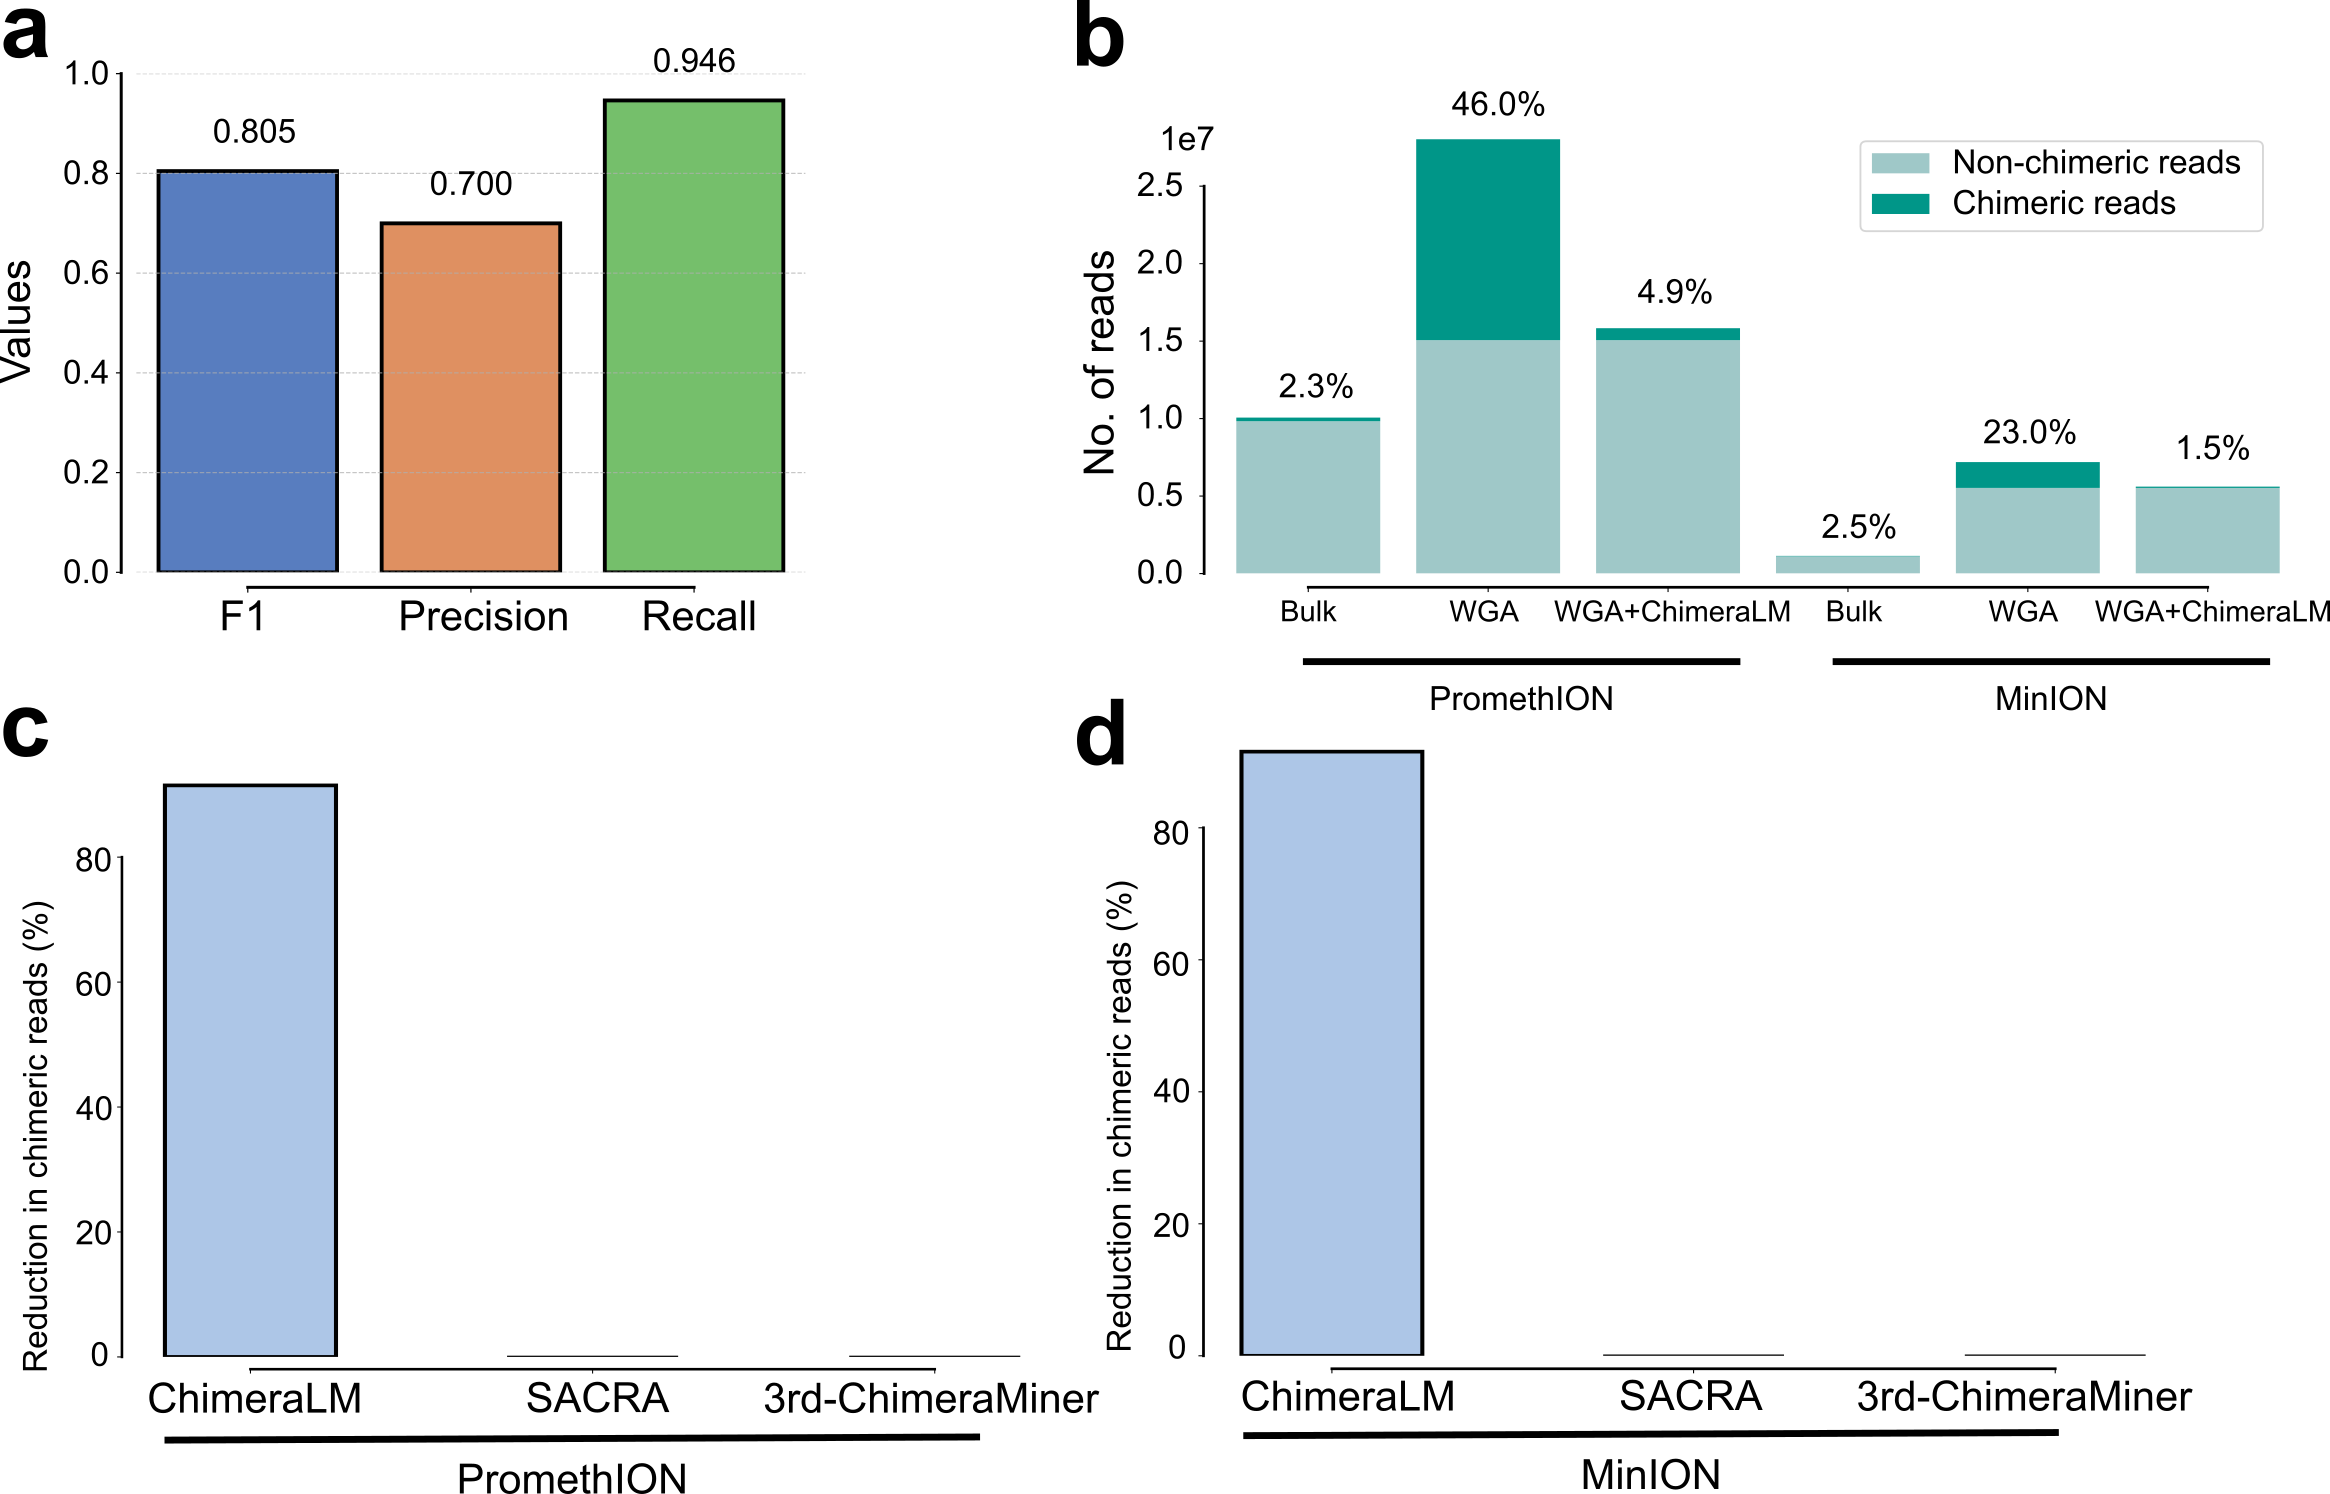
\includegraphics[width=0.95\textwidth]{final_figures/figure2}
	\end{center}
	\caption{Problem and Model}\label{fig:figure2}
\end{figure}


\begin{figure}
	\begin{center}
		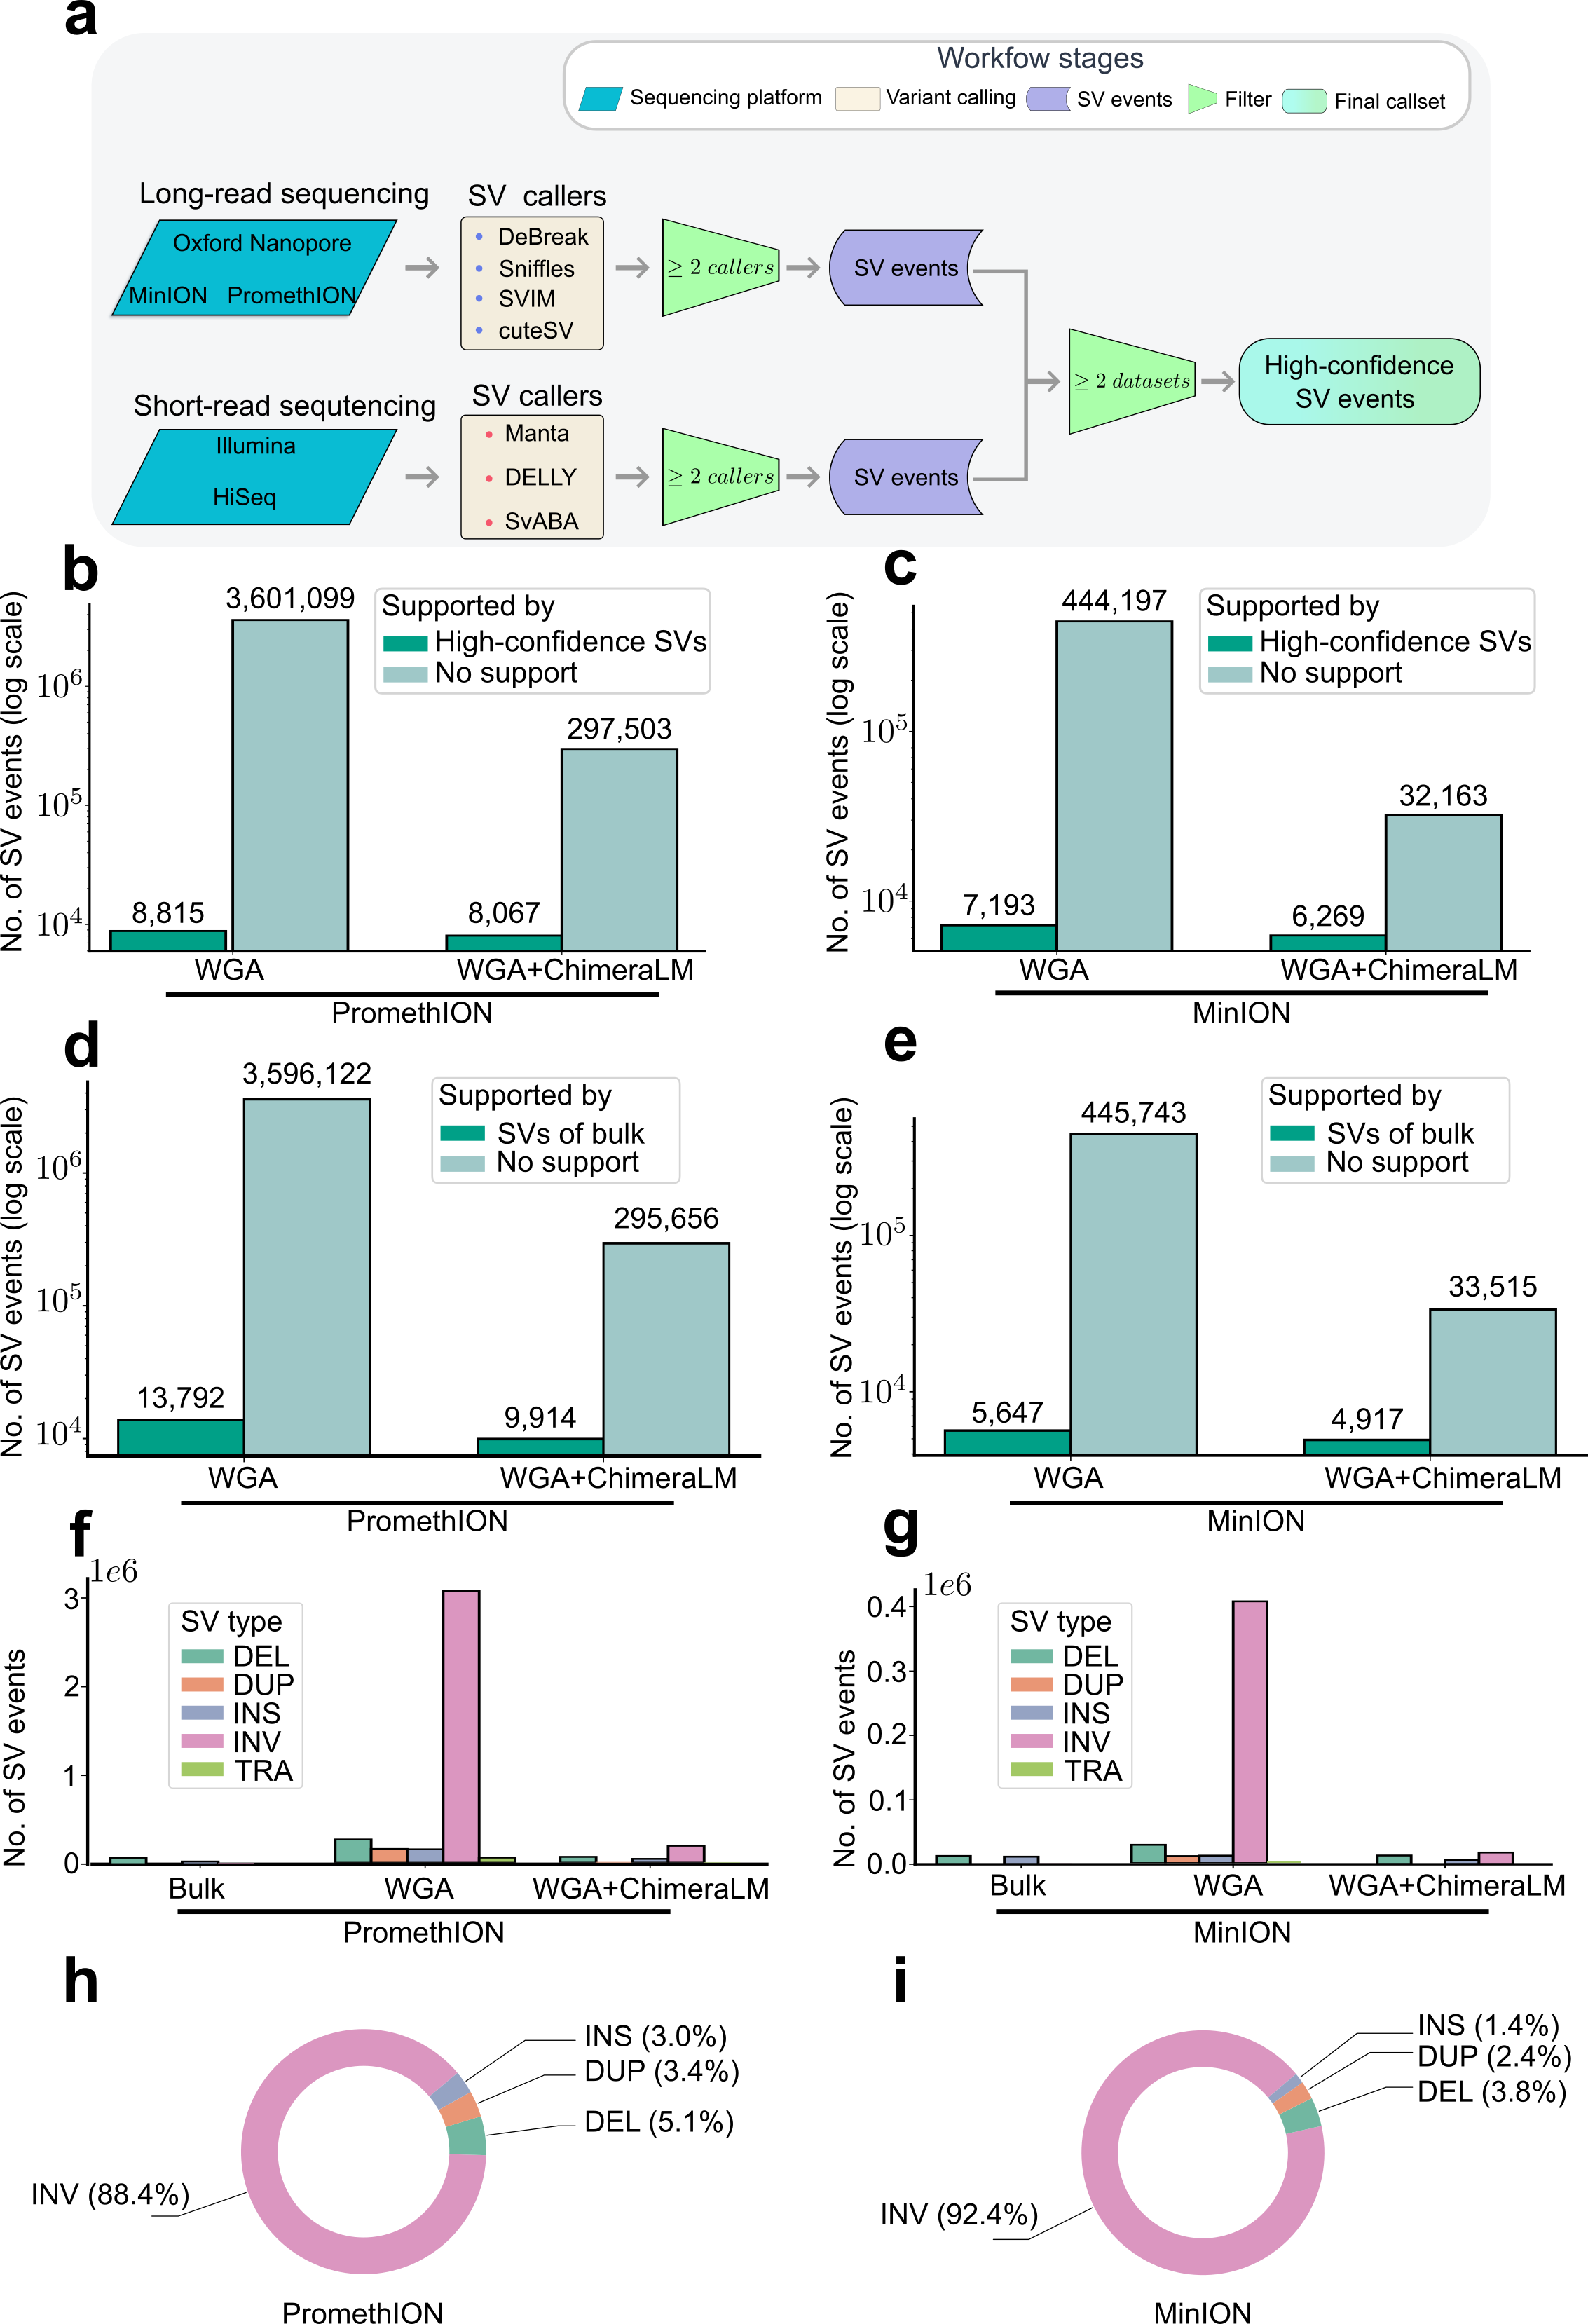
\includegraphics[width=0.95\textwidth]{final_figures/figure3}
	\end{center}
	\caption{Problem and Model}\label{fig:figure3}
\end{figure}

\section{Methods}\label{sec12}




\backmatter

\bmhead{Supplementary information}


\begin{figure}
	\begin{center}
		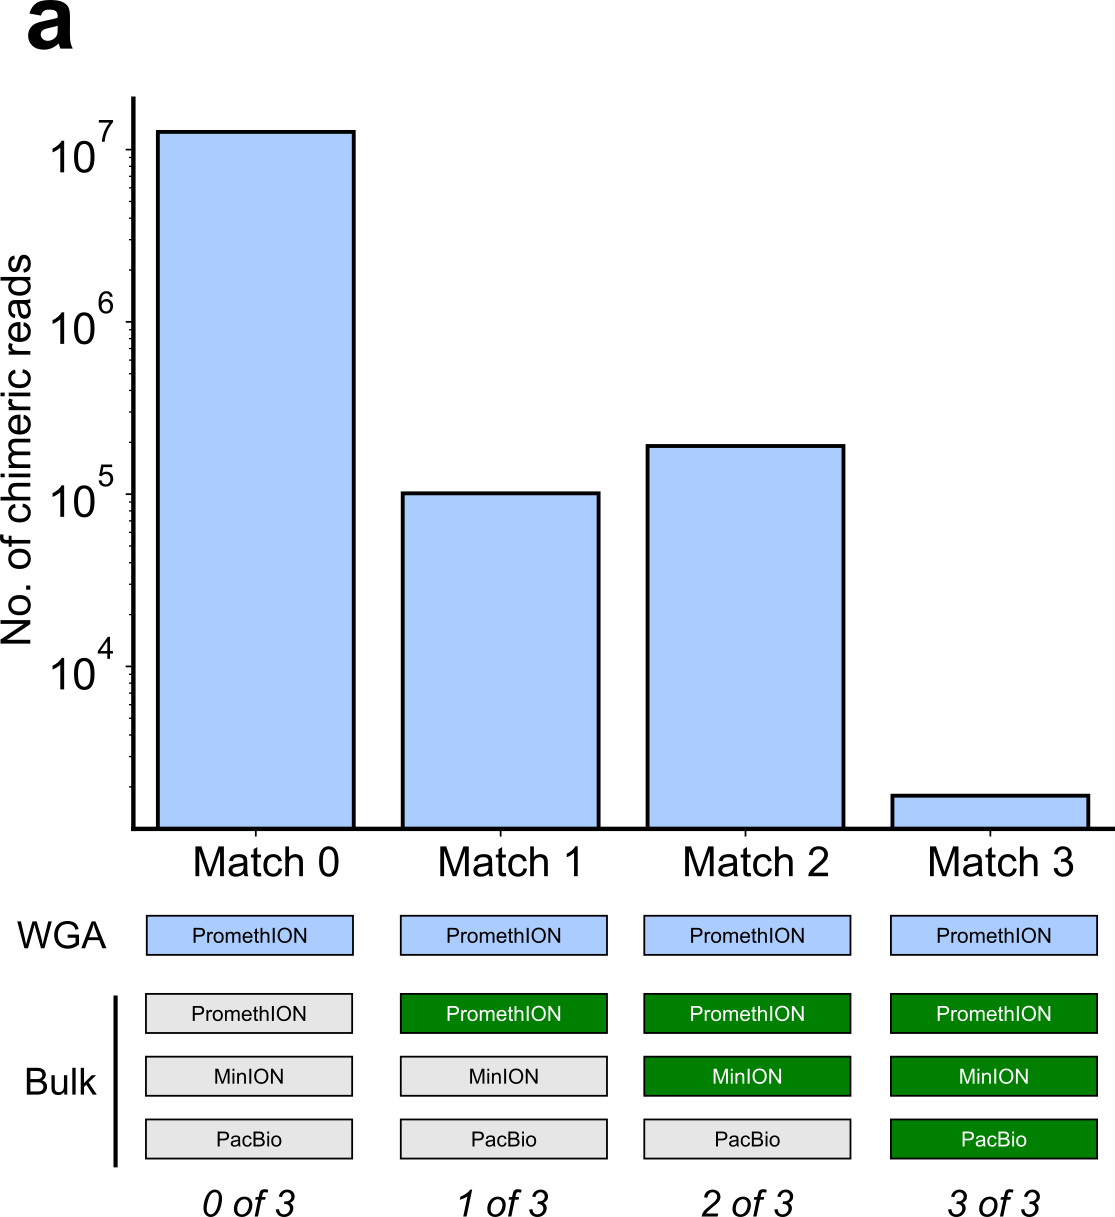
\includegraphics[width=0.95\textwidth]{final_figures/sf1}
	\end{center}
	\caption{Problem and Model}\label{fig:sf1}
\end{figure}


\begin{figure}
	\begin{center}
		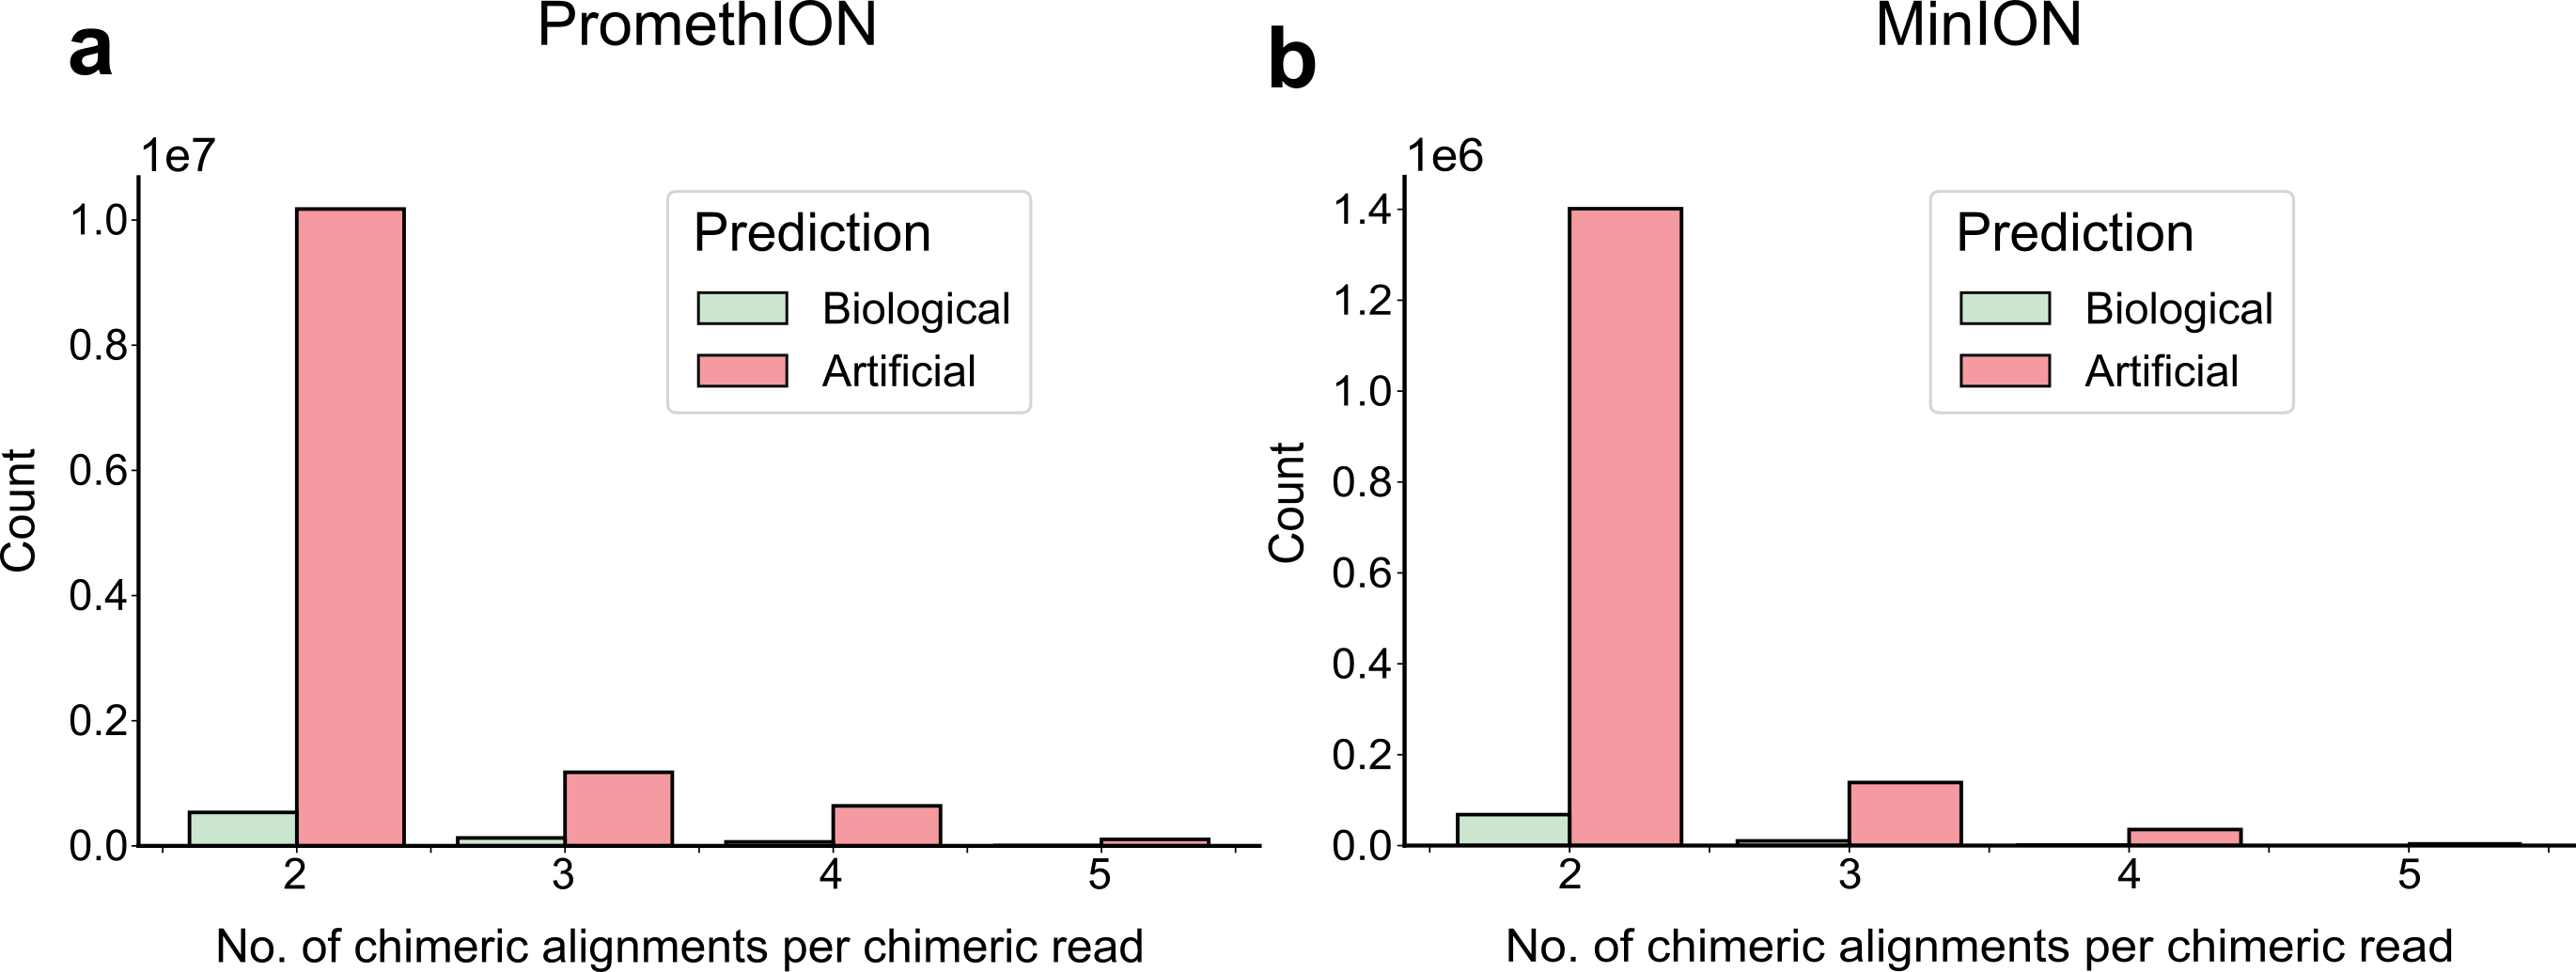
\includegraphics[width=0.95\textwidth]{final_figures/sf2}
	\end{center}
	\caption{Problem and Model}\label{fig:sf2}
\end{figure}

This separation aligns with how many transcript assembly algorithms work:

\begin{enumerate}[leftmargin=*]
	\item First, chains of exons and splice junctions are identified from the data
	\item Then, potential transcripts are derived by traversing the graph in different ways
	\item Finally, relationships between different transcript graphs are established
\end{enumerate}

\bmhead{Acknowledgements}

Acknowledgements are not compulsory. Where included they should be brief. Grant or contribution numbers may be acknowledged.

Please refer to Journal-level guidance for any specific requirements.

\section*{Declarations}

Some journals require declarations to be submitted in a standardised format. Please check the Instructions for Authors of the journal to which you are submitting to see if you need to complete this section. If yes, your manuscript must contain the following sections under the heading `Declarations':

\begin{itemize}
	\item Funding
	\item Conflict of interest/Competing interests (check journal-specific guidelines for which heading to use)
	\item Ethics approval and consent to participate
	\item Consent for publication
	\item Data availability
	\item Materials availability
	\item Code availability
	\item Author contribution
\end{itemize}

\noindent
If any of the sections are not relevant to your manuscript, please include the heading and write `Not applicable' for that section.

\begin{flushleft}%
	Editorial Policies for:

	\bigskip\noindent
	Springer journals and proceedings: \url{https://www.springer.com/gp/editorial-policies}

	\bigskip\noindent
	Nature Portfolio journals: \url{https://www.nature.com/nature-research/editorial-policies}

	\bigskip\noindent
	\textit{Scientific Reports}: \url{https://www.nature.com/srep/journal-policies/editorial-policies}

	\bigskip\noindent
	BMC journals: \url{https://www.biomedcentral.com/getpublished/editorial-policies}
\end{flushleft}

\begin{appendices}

	\printglossaries

	\section{Section title of first appendix}\label{secA1}

	An appendix contains supplementary information that is not an essential part of the text itself but which may be helpful in providing a more comprehensive understanding of the research problem or it is information that is too cumbersome to be included in the body of the paper.

	%%=============================================%%
	%% For submissions to Nature Portfolio Journals %%
	%% please use the heading ``Extended Data''.   %%
	%%=============================================%%

	%%=============================================================%%
	%% Sample for another appendix section			       %%
	%%=============================================================%%

	%% \section{Example of another appendix section}\label{secA2}%
	%% Appendices may be used for helpful, supporting or essential material that would otherwise
	%% clutter, break up or be distracting to the text. Appendices can consist of sections, figures,
	%% tables and equations etc.

\end{appendices}

%%===========================================================================================%%
%% If you are submitting to one of the Nature Portfolio journals, using the eJP submission   %%
%% system, please include the references within the manuscript file itself. You may do this  %%
%% by copying the reference list from your .bbl file, paste it into the main manuscript .tex %%
%% file, and delete the associated \verb+\bibliography+ commands.                            %%
%%===========================================================================================%%

\bibliography{sn-bibliography}% common bib file
%% if required, the content of .bbl file can be included here once bbl is generated
%%\input sn-article.bbl

\end{document}
